\documentclass[prb,twocolumn,9pt]{revtex4-1}

% LOAD PACKAGES

% GENERAL PACKAGES
\usepackage{graphicx}
\usepackage{wrapfig}
\usepackage{color}
\usepackage{latexsym,amsmath}
\usepackage{physics}
\usepackage{chemformula}
\usepackage{tabularx}
\usepackage{float}
\usepackage{siunitx}
\usepackage{amssymb}
%\usepackage[caption=false, justification=right]{subfig} % rovina la formattazione delle figure se caption=true
\usepackage[caption=false]{subfig}
\usepackage{multirow}

% LISTING PACKAGES
\usepackage{xcolor}
\usepackage{listings}
\usepackage{framed}
\usepackage{inconsolata} % To change the listing font

% URL PACKAGE AND SETTING
\definecolor{linkcolor}{rgb}{0,0,0.65} %hyperlink
\definecolor{linescolor}{rgb}{0.65,0.16,0.16}
\definecolor{cool}{RGB}{49,54,149}
\definecolor{hot}{RGB}{165,0,38}
\usepackage[pdftex,colorlinks=true, pdfstartview=FitV, linkcolor= linescolor, citecolor= linescolor, urlcolor= linkcolor, hyperindex=true,hyperfigures=true]{hyperref} %hyperlink%

% PAGE SETTING
\usepackage{fancyhdr} 

\pagestyle{fancyplain}
\fancyhf{}
\renewcommand{\headrulewidth}{0pt}
\fancyfoot[R]{\textbf{\thepage}}
%\fancyfoot[L]{Università degli Studi di Padova - Dipartimento di Fisica e Astronomia Galileo Galilei} 
%\fancyhead[L]{\textbf{Advanced Physics Laboratory Report}}
%\fancyhead[L]{\ifnum\value{section}>0\nouppercase{\textbf{\leftmark}\fi}}
%\fancyhead[R]{\textbf{Name1 Surname1 - Name2 Surname2}}
%\renewcommand{\headrulewidth}{0.2pt}
%\renewcommand{\footrulewidth}{0.1pt}

%\setlength\parindent{9pt} % To adjust the intendation

% SECTION STYLE
%Redefine \thesubsection as \thesection.\alph{subsection}. (\alph replaces the default \arabic; you could also choose, e.g., \Alph, \roman, and \Roman.)
\renewcommand{\thesection}{\textbf{\Roman{section}}}
\renewcommand{\thesubsection}{\textbf{\arabic{subsection}}}
\renewcommand{\thesubsubsection}{\textbf{\Alph{subsubsection}}}
%\renewcommand{\thesection}{\textbf{\arabic{section}}}
%\renewcommand{\thesubsection}{\thesection.\textbf{\arabic{subsection}}}
%\renewcommand{\thesubsubsection}{\textbf{\thesection.\arabic{subsection}.\arabic{subsubsection}}}

% FIGURE AND TABLE STYLE
\renewcommand{\tablename}{\textbf{TAB.}}
\renewcommand{\thetable}{\textbf{\arabic{table}}}

% ELIMINARE COMMENTO NELLA COMPILAZIONE FINALE
%\renewcommand{\figurename}{\textbf{FIG.}}
%\renewcommand{\thefigure}{\textbf{\arabic{figure}}}

% BIBLIOGRAPHY FILE AND SETTING
\bibliographystyle{aipnum4-1}
\setcitestyle{numbers,square}

%\usepackage[backend=biber, sorting=ynt]{biblatex}
%\addbibresource{references.bib}


\begin{document}



% FRONTESPIZIO

% Title
\title{Spatial monitoring of anti-vaccine opinions through Twitter: a method proposal}



\author{Rachele Favaretto}
\author{Alessandro Lambertini}
\author{Alice Pagano}

\date{\today}

% Abstract
\begin{abstract}

Vaccines are a central topic in public debate and the spreading of novax opinions on social networks have a relevant influence in vaccination hesitancy. 
In this context, a quantitative modelling of this phenomenon could help to organize more effective and less dispersive national vaccination plans.
In this work, we develop a method to extract a spatial distribution of novax opinions from Twitter. In particular, we exploit it to analyze anti-vaccine opinions distribution in Italy in the time window spacing from 2017 to 2020 at a region level. 
We observe the impact on Twitter activity of the Covid-19 pandemic.
Moreover, for a fixed year, we investigate a possible correlation between novax ideas distribution and measles vaccination coverage. However, due to poor statistic, we observe no correspondence between low vaccination coverage and novax hubs. 
Nonetheless, mining and localizing opinions from social networks could have a great relevance, because it can be useful in identifying hubs of anti-vaccination ideas and consequently in choosing where to invest resources for public opinion awareness campaigns on vaccination.

\end{abstract}


% Make title
\maketitle



\section{Introduction}
\label{sec:introduction}

In the last months, in particular after the administration of the first doses of the Covid-19 vaccine, vaccination has become a central topic in public debate on social networks, where people feel free to express their viewpoints or doubts about it. For this reason, social networks are useful tools to monitor people's mood, ideas and opinions. In Italy, from January 2017 to January 2020, the number of the active users of social networks have grown from 31 to 35 million, with a constant average daily usage of around 2 hours. In the same time interval, in particular, Twitter users have grown from 7.8 to 11.9 million, so they can be considered a quite large sample of the Italian population (60 million) \cite{Users}.
Given these huge numbers, it is easy to understand that rumors and disinformation regarding vaccines can be widely diffused in social networks, resulting determinant on the loss of trust in vaccination and consequently in hesitation to be vaccinated. In Italy, vaccine hesitancy, defined as “delay in acceptance or refusal of vaccination despite the availability of vaccination services”, become so diffuse that led to an alarming drop in vaccination coverage since 2013 \cite{twitter_sentinel}. Low coverage made an immunization prevention plan necessary: on 28 July 2017 became law the Lorenzin Decree on vaccines which makes 10 vaccinations mandatory, including measles vaccination, for minors between the ages of 0 and 16; the vaccinations are also binding for registration in kindergartens \cite{ministerosalute}. This restriction has contributed in making the discussion on vaccines a hot topic in social networks in that period.
As said before, also in 2020, the year of the Covid-19 pandemic, debate on vaccination is central in social networks: the vaccine research and the administration of the first doses of vaccine triggered the novax and also other people who were not novax before. On the contrary, others became more sensitive to the importance of vaccines, in the light of the effects of a disease that can not be stopped by vaccines yet.

In this article, we analyze the distribution of novax opinions in Italy, using tweets with clearly anti-vaccine content. We collect tweets and retweets in the time interval 2017-2020 and have a first overview of them making a semantic analysis. The collected tweets are shared only by users who indicate their geographical origin in their profile. Through this information, indeed, we make a geographical map of novax opinions in Italy. The coarse graining level of our analysis stops to the region level. We study the anti-vaccination opinion distribution to see if it is homogeneous, or if there are hubs of novax people. Moreover, we observe if the distribution has changed over the years. In particular, we make a comparison between the pre-pandemic years 2017-2019 and 2020 to investigate if the novax Twitter users have changed due to Covid-19.
Finally, we compare the distribution of the novax opinions with the measles vaccination coverage in the same years, trying to find a correspondence between low coverage and novax hubs. 


\section{Methods}
\label{sec:methods}

\subsection{Anti-vaccination tweets selection and preprocessing}
\label{sec:Anti-vaccination tweets selection and preprocessing}

A dataset of tweets from January 2017 to December 2020 is collected using hashtags related to anti-vaccination movements and, for this purpose, the full archive search of Twitter API is exploited. 
More specifically, for each month, we make a request with the Twitter API by filtering through Italian hashtags such as “$\#$iononmivaccino” or “$\#$libertàdiscelta”. However, because of the limited number of requests at our disposal, a maximum of 100 tweets can be extracted for each month.
Moreover, for each tweet, we store only the most relevant information which will be useful in our analysis as the tweet text and id or the user location information.

The collected data are processed in order to associate to each tweet its source location taken from the user location field, if present. Otherwise, the tweet is rejected. In particular, to extract meaningful information from it, we develop a Python script which compare the text with a list of all Italian cities, provinces, regions and provinces' initials by means of regex. At the end, for each year under analysis, we obtain a dataset of dimension $d_t$ (Tab. \ref{tab:dataset_dimension}) where each tweet is associated to an Italian region and to geographical coordinates which correspond to the region capital. The error associated to the tweet-region classification algorithm turns to be of around $3\%$. 

After that, each tweet text is manually analyzed in order to verify if it is really expressing a novax opinion, otherwise the tweet is not considered in the further analysis. The dimension of the dataset after this preprocessing is referred as $d_{nv}$ (Tab. \ref{tab:dataset_dimension}). Moreover, a semantic analysis of novax tweets content is performed by filtering the tweet text by a list of common stop-words (Fig. \ref{fig:count_word}).


Of course there are several limitations in this analysis. The first one is given by the geolocalization of the tweets. Indeed, we can assign a region of provenience only to a small percentage of the collected tweets ($25\%$) since most of the users decide to keep their location private \cite{disease_prevention_review}. Moreover, as already mentioned, for each API request we can access only to a maximum number of 100 tweets (or retweets, we could not filter only for tweets) and we had also a limited number of requests at our disposal. This leads to small statistic in our analysis. However, in principle this problem can be solved with a premium account.
Another issue of this method would be the manual classification of tweets. As a matter of fact, for this analysis, due to the poor statistic, the manual classification is not challenging. However, in principle, one could extend this method also for analyzing large statistic scenario. In this case, a valid solution could be training a neural network for classifying novax opinion \cite{twitter_sentinel}.

\subsection{User overlap over years}
\label{sec:User overlap over years}

We study the correlation of users over the years from 2017 to 2020 in order to investigate the influence of Covid-19 in triggering novax opinions. In particular, as a correlation measurement we take the overlap of the same users for the different years in the anti-vaccination dataset (Sec. \ref{sec:Anti-vaccination tweets selection and preprocessing}). In more details, to represent this we use a generalization of a Venn diagram (Fig. \ref{fig:overlap}).


\subsection{Region weights from tweets}
\label{sec:Region weights from tweets}

An analysis of the spatial distribution of novax tweets is performed. 

First of all, we associate a weight $w_i$ to each tweet given by 
\begin{equation}
    w_i = \frac{1 + N_{f} + 5 N_{r}}{A_i}
    \label{eq:weight}
\end{equation}
where $N_f$ is the favourite count and $N_r$ is the number of retweets associated to the tweet ($N_r$ is considered null if the tweet is already a retweet). The normalization factor $A_i$ is the activity of the region associated to a tweet (see Sec. \ref{sec:Monitor twitter activity of Italian regions}). 
The idea at the basis of this classification is that more likes or number of retweets a tweet has, the greater is its influence on the opinion of other individuals. Instead, the greatest is the region activity, the weaker is the relevance of the tweet. 

After that, a weight $W_u$ is associated to each user by summing the weights $w_i$ associated to all its tweets. Hence, we obtain novax individuals whose degree in spreading antivaccine information is $W_u$. In this step, the dataset is filtered trough unique users and its size $d_u$ is even smaller (Tab. \ref{tab:dataset_dimension}).

Finally, we assign a weight $W_r$ to each Italian region considering the sum of all the users belonging to it. 


\subsection{Monitor twitter activity of Italian regions}
\label{sec:Monitor twitter activity of Italian regions}
In order to compute the normalization factor $A_i$ in Eq. \eqref{eq:weight}, a dataset of geolocalized tweets obtained from the Italian Twitter stream in the first two weeks of January 2021 is collected. In particular, a region of provenience is associated to each tweet following the same procedure of Sec. \ref{sec:Anti-vaccination tweets selection and preprocessing}. 

Then, the dataset is filtered trough unique user and for each region the number of active user $N_{a_i}$ is computed. A percentage of activity $A_i = \frac{ N_{a_i} \cdot 100}{ \sum_i N_{a_i} } $ is associated to each region $i$. 

The concept at the basis of this dataset construction is that, in order to further associate a weight to spatial distribution of novax tweets, we need the information regarding the distribution activity of Twitter in Italy.
For instance, if in one region Twitter is less used than in another one, the tweets collected from that region will have a greater importance in novax analysis.  

For the whole paper, these percentages of spatial Twitter activity in Italy will be considered unchanged over the years, even if this stream analysis is restricted only to the first few weeks of January. This is a very stringent assumption that need to be taken into account in the analysis of our results. However, it is unavoidable since a more sophisticated analysis would require more time and more available resources.
In addition, another limitation is given by the tweet geolocalization as already discussed in Sec. \ref{sec:Anti-vaccination tweets selection and preprocessing}.


\subsection{Vaccination data}
\label{sec:Vaccination data}
Measles vaccination coverage in the years 2017-2019 divided by region are collected from the Italian Ministry of Health \cite{ministerosalute}. The cohorts considered are children born in 2015-2017 (vaccination coverage two years after birth).
This time window is chosen in order to have data resulting from the most recent choices of new parents, which are more consistent and relevant for the novax opinion of the years under analysis. Unfortunately, data for the year 2020 are not available yet. The collected data are shown in Tab. \ref{tab:vaxcoverage}.


\subsection{Visualization: map}
\label{sec:Visualization:map}
In order to visualize effectively our processed data, the maps shown in Fig. \ref{fig:map_result} are produced. These maps have been developed trough a Python script that exploit shapefiles representing regions and provinces of Italy \cite{istat}.
The analysis is conducted at a region level, with the exception of Trentino Alto Adige. This region is divided into the two autonomous provinces, Trento and Bolzano, since they have two very different levels of vaccination coverage. For this reason, the two provinces are kept disjoined, hence we modify the region shapefile accordingly.

In these maps, we associate to every region a different shade of red, representing the vaccination coverage, and a blue point, whose radius is proportional to the novax activity $W_r$ measured in that regions as described in Sec. \ref{sec:Region weights from tweets}.

%\subsection{Visualization: most common words}
%\label{sec:Visualization: most common words}
%By means of a Python script, we highlight the most common words found in the texts of the different tweets. In order to clean up the content of each tweet from meaningless words for the purposes of our analysis, the texts are filtered by a list of common stop-words. In Fig.\ref{fig:count_word} a bar-plot with the result of this analysis is shown.

\section{Results}
\label{sec:results}

In Tab. \ref{tab:dataset_dimension} the dataset dimension at the different steps of processing is reported.

 \begin{table}[b]
    \begin{minipage}[l]{1.0\columnwidth}
    \centering
        \begin{tabular*}{\linewidth}{@{\extracolsep{\fill}}
        l cccc 
        }
       %\toprule
            & \textbf{2017} & \textbf{2018} &  \textbf{2019} & \textbf{2020} \\
        \colrule
            $\pmb{d_t}$    & 438 & 405 & 382 & 277 \\
       % \colrule
            $\pmb{d_{nv}}$ & 83.3 \% & 88.6 \% & 98.2 \% & 82.3 \% \\
       % \colrule
            $\pmb{d_{u}}$  & 22.5 \% & 32.3 \% & 39.2 \% & 59.2 \% \\
       %\botrule
        \end{tabular*}
    \caption{Dataset dimension for the different years under study. $d_t$ is the total dimension of the tweet dataset after location classification. $d_{nv}$ is the percentage of $d_t$ of tweets that express actually a novax opinion. $d_u$ is the percentage of unique users of $d_{nv}$. }
    \label{tab:dataset_dimension}
    \end{minipage}
    \end{table}
    
\noindent First of all, we note that the tweet dataset dimension $d_t$ is very low from the beginning of the analysis ($\sim 400$ tweets for each year). This is due to the several limitations already discussed in Sec. \ref{sec:Anti-vaccination tweets selection and preprocessing}.
Then, the dimension is further reduced by the manual classification of the tweet text. Indeed, only a percentage $d_{nv}$ of the collected tweets express actually a novax opinion. We can note that this percentage is not constant over the years. The main discrepancy can be attached to the chosen hashtags: we use the same hashtags for all the investigated years, however, hashtags are highly correlated to the year of interest. For example, the hashtag “$\#$libertàdiscelta”, depending on the period, includes also several not novax tweets: in the first months of 2017 it is used in tweets pro-euthanasia, while in May and June 2020 it is present in many posts about freedom of religious faith. These two years, indeed, results to be the ones with lowest $d_{nv}$ percentage.
These non negligible stochastic fluctuations in the dimension of the dataset are emphasized by the poor statistics: the tweets selection enable us to select only 100 random tweets for each month with the given hashtags. 

\begin{figure}[t]
   \begin{minipage}[l]{1.0\columnwidth}
   \centering
   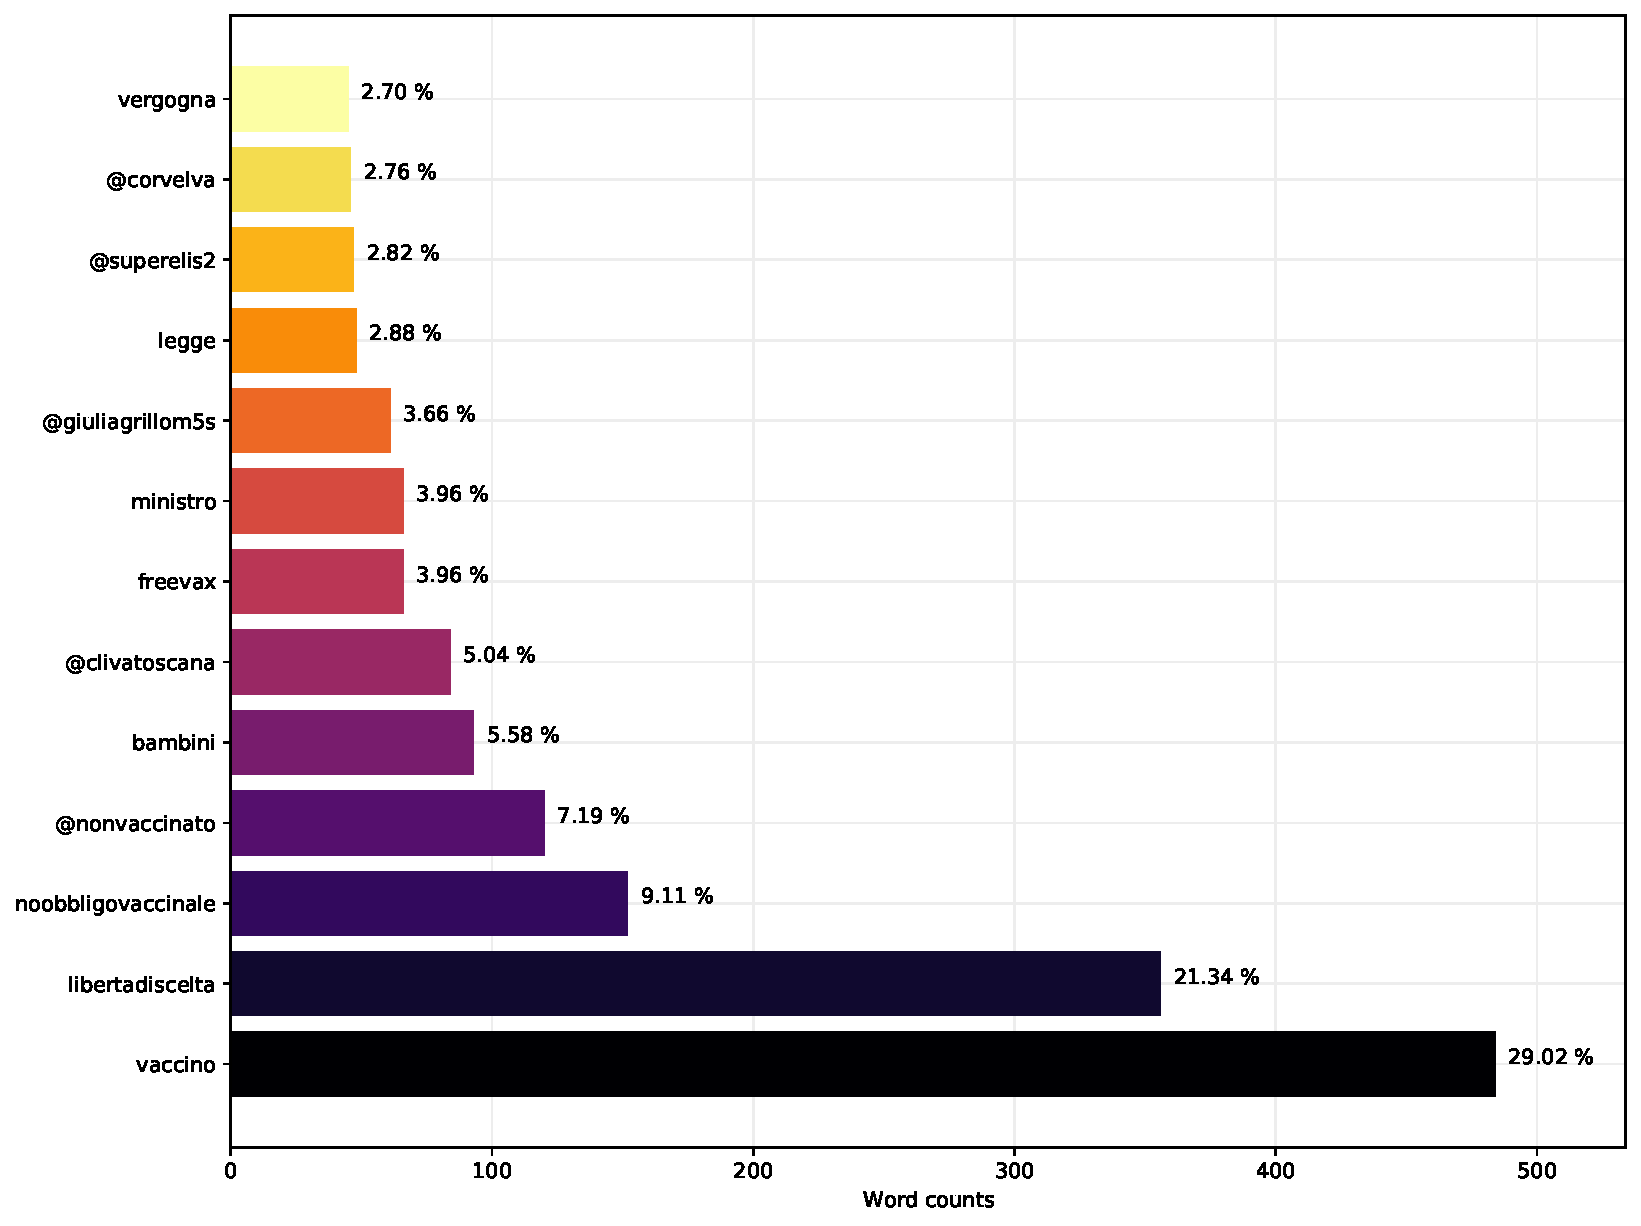
\includegraphics[width=1\textwidth]{Paper_template/image/word_2017-2020.pdf}
   \caption{Histogram of most used words in the novax collected tweets in 2017-2020 time interval.}
   \label{fig:count_word}
   \end{minipage}
\end{figure}

To make a first overview of the novax tweets, we carried out a semantic analysis as mentioned in Sec. \ref{sec:Anti-vaccination tweets selection and preprocessing}. Fig. \ref{fig:count_word} shows a histogram with the most common words in the collected novax tweets of the four years 2017-2020. We do not notice relevant differences between the years, so we only report the total histogram. Obviously, the most frequent words are “vaccino” (vaccine), “libertadiscelta” (freedom of choice) and “noobbligovaccinale” (no obligatory vaccine), being these the hashtags through which we searched for the tweets.
Moreover, there are two openly novax association accounts (“@clivatoscana” from Toscana and “@corvelva” form Veneto) and single users (“@nonvaccinato” and “@superelis2”) which are among the recurring words: they are the main producers of novax contents that are retweeted by other users who limit themselves to passive sharing (retweets) and not to create original tweets. Therefore, these content creators can be considered real super spreaders. On the other hand, “@giuliagrillom5s” account is a popular word because she was the health minister (“ministro” is another frequently used word) for most of the period under analysis. Similarly, the name of the former health minister Beatrice Lorenzin was recurring in 2017 tweets.

\begin{figure}[t]
   \begin{minipage}[l]{1.0\columnwidth}
   \centering
   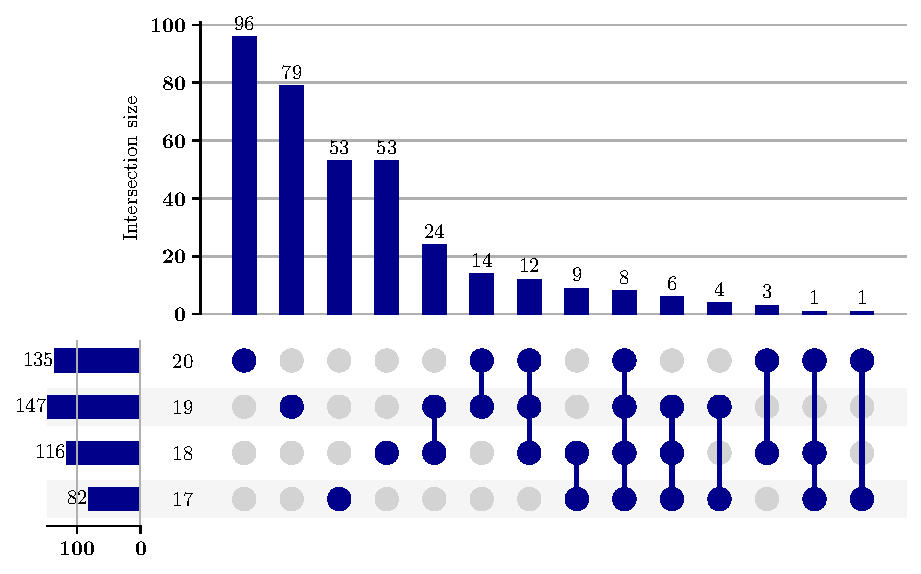
\includegraphics[width=1\textwidth]{Paper_template/image/user_overlap/overlap.pdf}
   \caption{Twitter user overlap between 2017, 2018, 2019 and 2020. Every blue dot indicates the concerned year. Then, the top bar chart tells that for the given year, we have that many users. Two or more connected dots, indicate user that have tweeted in multiple years. On the bar chart on the left, the dimension $d_u$ of the dataset for each year is reported.
   }
   \label{fig:overlap}
   \end{minipage}
\end{figure}

After that, we filter the tweets trough unique users and the dataset dimension results dramatically reduced. It means that on average we have more or less 4-5 tweets associated to the same user. Interestingly, the percentage $d_u$ is increasing over the years. In particular, in 2020 $d_u$ reaches a peak of $\sim 59 \%$ of $d_{nv}$ (Tab. \ref{tab:dataset_dimension}). It is possible that the Covid-19 pandemic makes conscious citizens of vaccination dynamics and has influenced different people to express their opinion. 

The high number of unique users of 2020, most of them also different from the other years, is evident in Fig. \ref{fig:overlap}, where the correlation between Twitter novax user over the years is illustrated. 
Furthermore, the correlation between consecutive years is higher than the others. For instance, it is possible that the same user have been tweeting for a couple of years and then he stops.



 \begin{table}[b]
    \begin{minipage}[l]{1.0\columnwidth}
    \centering
        \begin{tabular*}{\linewidth}{@{\extracolsep{\fill}} c c c c}
       \textbf{Region}	&	\textbf{$I$}	&	\textbf{$A$} &	\textbf{$\frac{I- A}{I}$}	\\
 \colrule
Prov. Au. di Bolzano	&	0.9	&	0.2	&	0.7	\\
Molise	&	0.5	&	0.2	&	0.6	\\
Sicilia	&	8.2	&	5.5	&	0.3	\\
Puglia	&	6.6	&	4.5	&	0.3	\\
Prov. Au. di Trento	&	0.9	&	0.6	&	0.3	\\
Calabria	&	3.2	&	2.3	&	0.3	\\
Campania	&	9.6	&	7.3	&	0.2	\\
Basilicata	&	0.9	&	0.7	&	0.2	\\
Friuli Venezia Giulia	&	2.0	&	1.6	&	0.2	\\
Veneto	&	8.2	&	6.6	&	0.2	\\
Abruzzo	&	2.2	&	1.8	&	0.2	\\
Sardegna	&	2.7	&	2.4	&	0.1	\\
Valle d'Aosta	&	0.2	&	0.2	&	0.1	\\
Piemonte	&	7.2	&	7.1	&	0.0	\\
Umbria	&	1.5	&	1.5	&	0.0	\\
Marche	&	2.5	&	2.7	&	-0.1	\\
Emilia Romagna	&	7.5	&	8.5	&	-0.1	\\
Lombardia	&	16.8	&	19.2	&	-0.1	\\
Toscana	&	6.2	&	7.5	&	-0.2	\\
Liguria	&	2.6	&	3.4	&	-0.3	\\
Lazio	&	9.7	&	16.0	&	-0.7	\\

        \end{tabular*}
    \caption{Percentage of inhabitants $I$ (at 1 January 2020 \cite{istat}) and Twitter activity $A$ of the Italian regions. Data are sorted in descending order according to the third column $\frac{I- A}{I}$ which quantifies how active a region is on Twitter compared to the number of inhabitants.}
    \label{tab:inhab-activity}
    \end{minipage}
    \end{table}

 \begin{table}[b]
    \begin{minipage}[l]{1.0\columnwidth}
    \centering
        \begin{tabular*}{\linewidth}{@{\extracolsep{\fill}} c c c c}
       \textbf{Region}	&	\textbf{2017}	&	\textbf{2018}	&	\textbf{2019}	\\
 \colrule							
Abruzzo	&	89.20	&	94.49	&	95.05	\\
Basilicata	&	92.90	&	92.98	&	92.57	\\
Calabria	&	92.79	&	92.72	&	93.08	\\
Campania	&	92.03	&	93.39	&	94.67	\\
Emilia Romagna	&	93.48	&	93.67	&	95.21	\\
Friuli Venezia Giulia	&	86.55	&	91.24	&	92.49	\\
Lazio	&	95.34	&	94.87	&	95.72	\\
Liguria	&	90.92	&	94.04	&	93.15	\\
Lombardia	&	93.92	&	94.16	&	95.56	\\
Marche	&	88.21	&	92.07	&	93.75	\\
Molise	&	90.48	&	91.95	&	93.39	\\
Piemonte	&	94.72	&	94.67	&	95.56	\\
Prov. Au. di Bolzano	&	71.86	&	70.84	&	75.53	\\
Prov. Au. di Trento	&	91.68	&	94.30	&	95.48	\\
Puglia	&	91.09	&	94.18	&	94.38	\\
Sardegna	&	93.00	&	92.33	&	93.61	\\
Sicilia	&	85.63	&	90.94	&	92.20	\\
Toscana	&	93.51	&	95.04	&	96.11	\\
Umbria	&	94.53	&	94.59	&	95.23	\\
Valle d'Aosta	&	90.33	&	91.43	&	91.54	\\
Veneto	&	92.34	&	93.49	&	95.12	\\
Italian average & 91.84 & 93.22 & 94.49 \\
        \end{tabular*}
    \caption{Measles vaccination coverage two years after birth in the years 2017-2019 divided by regions. The last line is the Italian average \cite{ministerosalute}.  }
    \label{tab:vaxcoverage}
    \end{minipage}
    \end{table}
 
As far as the stream dataset is concerned, in two weeks we collect around 48k geolocalized tweets of 7k unique users. This dataset has the big limitation of having been collected in just two weeks, so it could be very biased, as already mentioned in Sec. \ref{sec:Monitor twitter activity of Italian regions}.

To compute the percentage of the Twitter activity $A$ for each region, we considered the dataset filtered by unique users as explained in Sec. \ref{sec:Monitor twitter activity of Italian regions}.
Tab. \ref{tab:inhab-activity} shows $A$ compared to the number of inhabitants $I$ by region. The third column quantifies how active on Twitter a region is with respect to its number of inhabitants: the autonomous province of Bolzano is the least active, followed by Molise and most of the southern regions. Also North-East regions are less active than populated. On the contrary there are many Twitter users in Lazio, Liguria, Toscana, Lombardia and Emilia Romagna.


	% To insert four subfigure
	\begin{figure*}[t]
	\begin{minipage}[c]{0.49\linewidth}
	\centering
	\subfloat[][2017]{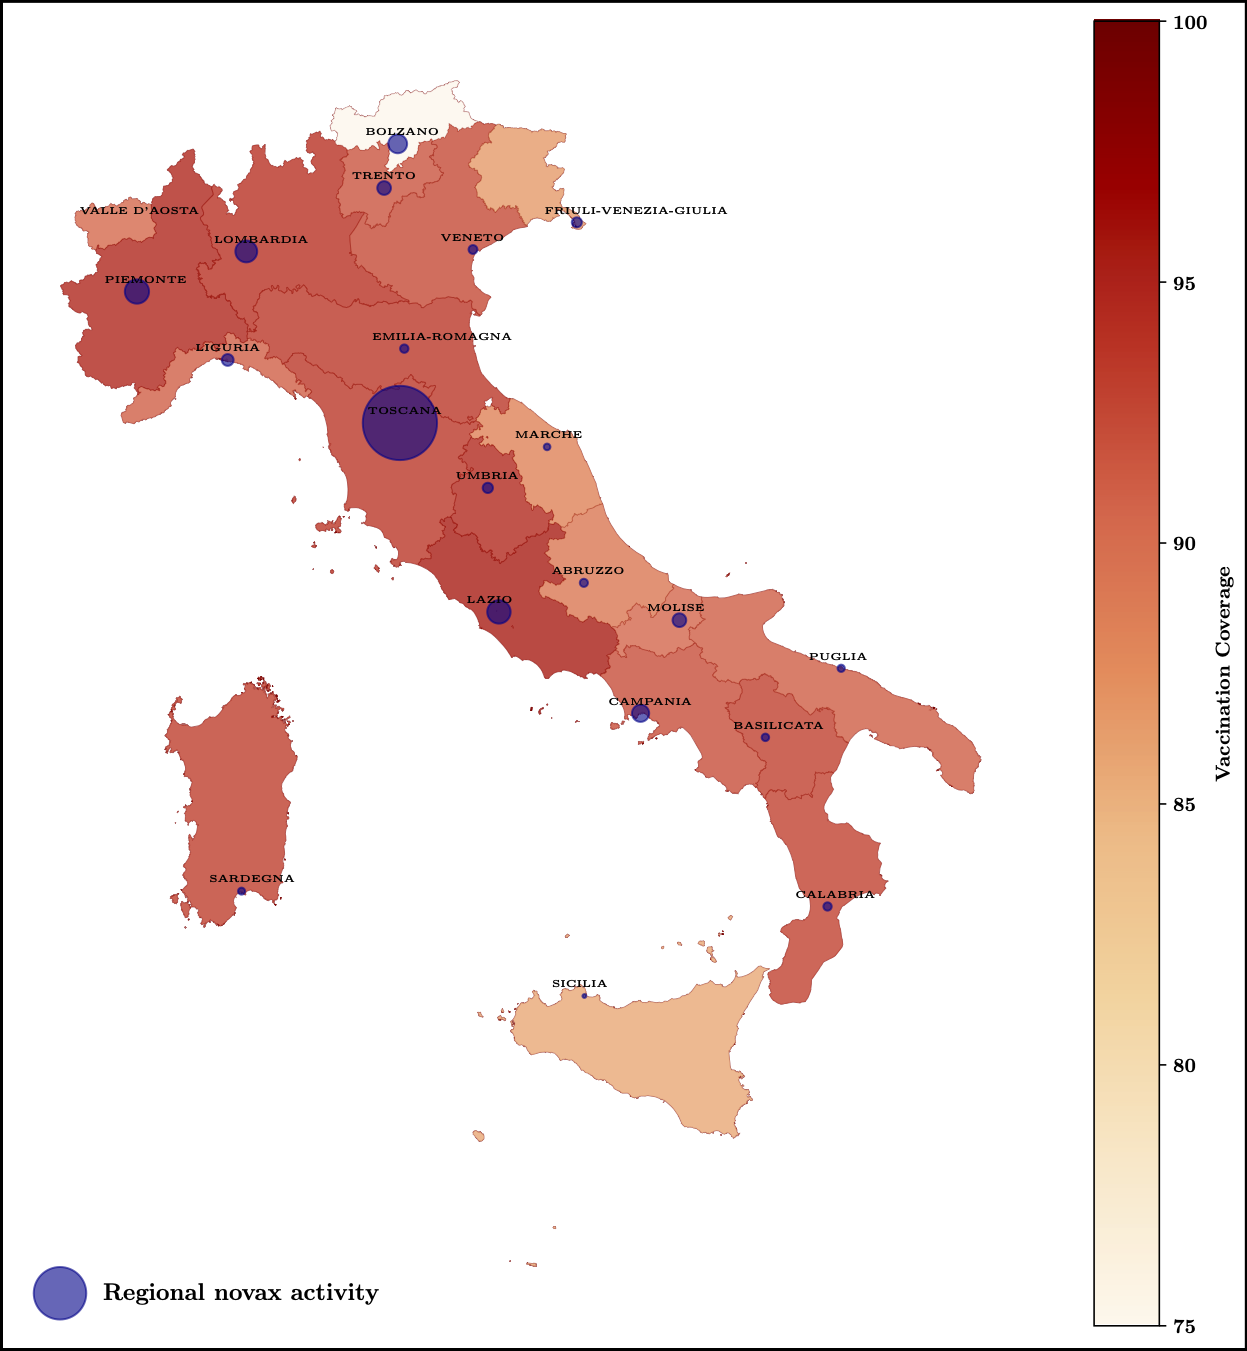
\includegraphics[width=0.8\textwidth]{Paper_template/image/map/map_2017.pdf} \label{fig:map_result_a} }
	\end{minipage}
	\begin{minipage}[]{0.49\linewidth}
	\centering
	\subfloat[][2018]{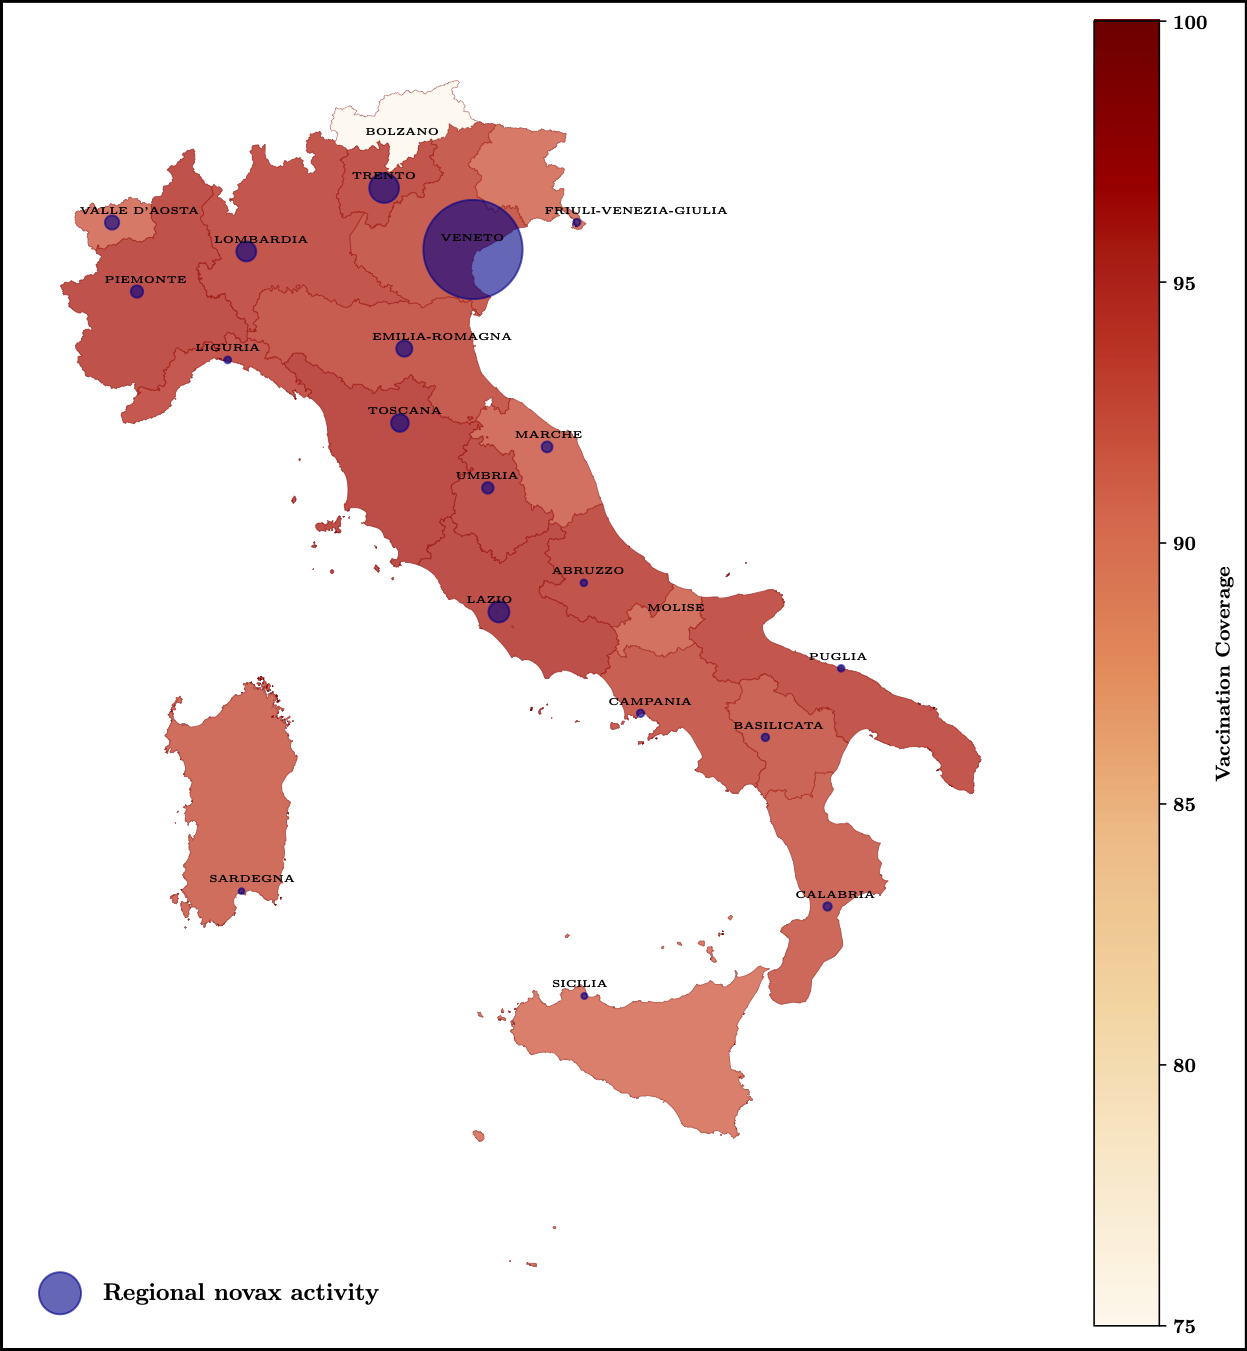
\includegraphics[width=0.8\textwidth]{Paper_template/image/map/map_2018.pdf} \label{fig:map_result_b} }
	\end{minipage} \\
	\vfill
	\begin{minipage}[c]{0.49\linewidth}
	\centering
	\subfloat[][2019]{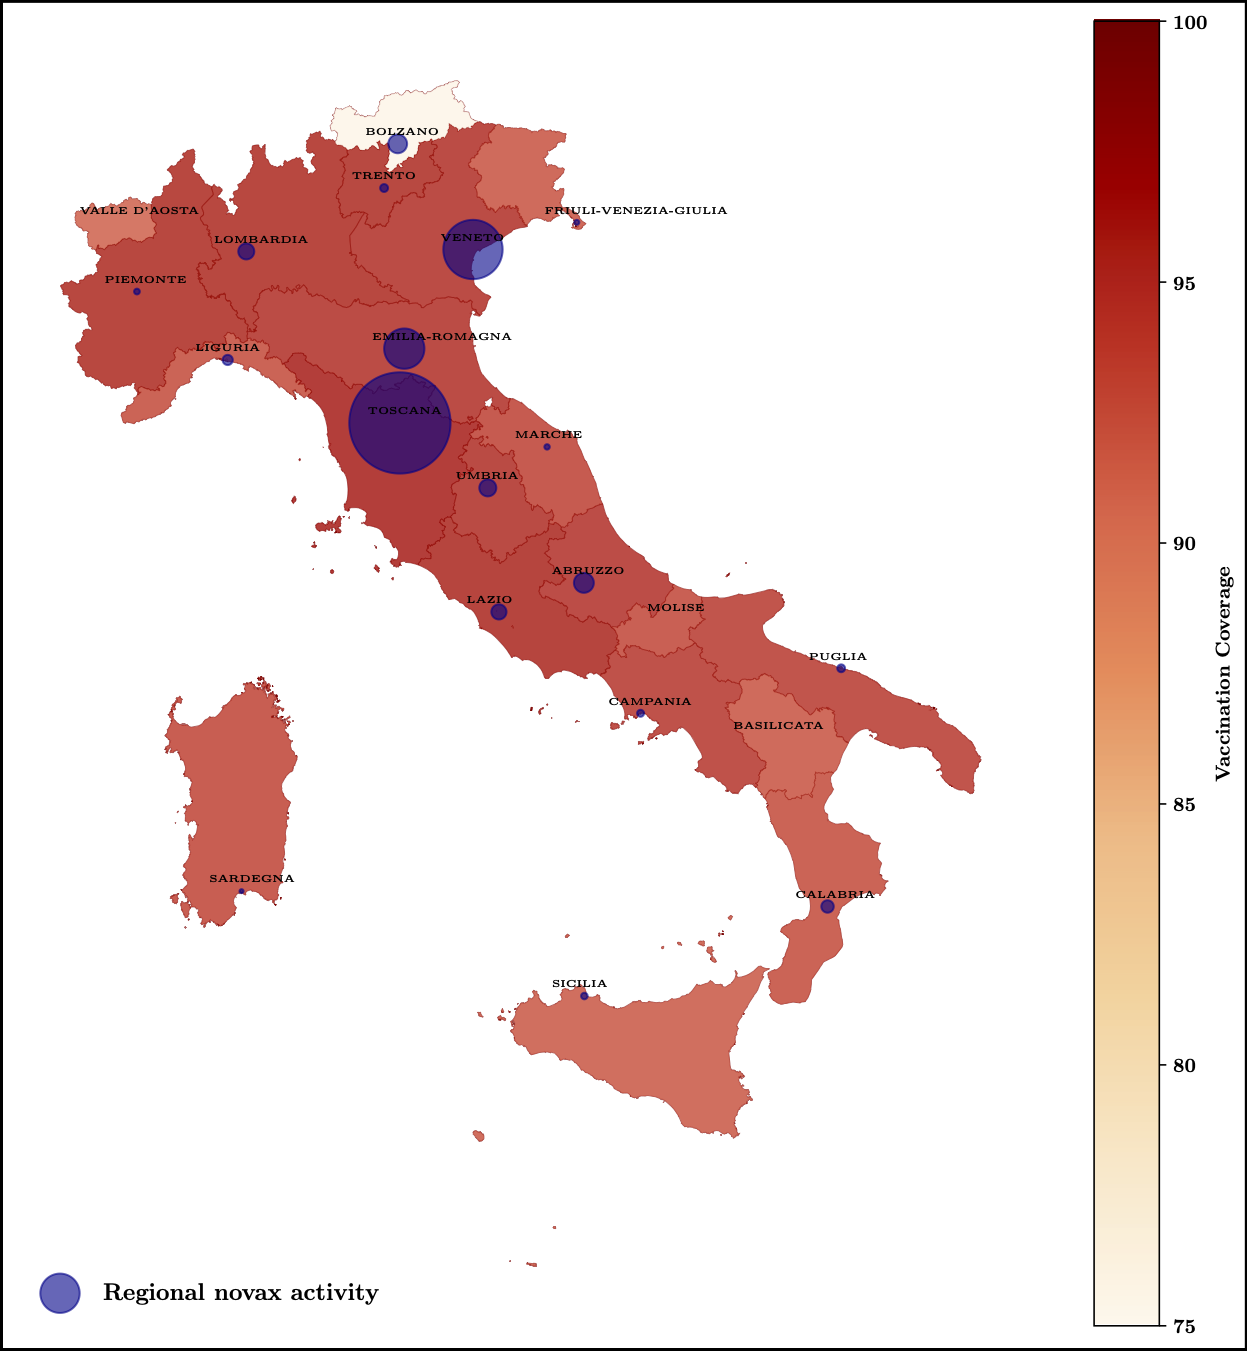
\includegraphics[width=0.8\textwidth]{Paper_template/image/map/map_2019.pdf} \label{fig:map_result_c} }
	\end{minipage}
	\begin{minipage}[]{0.49\linewidth}
	\centering
	\subfloat[][2020]{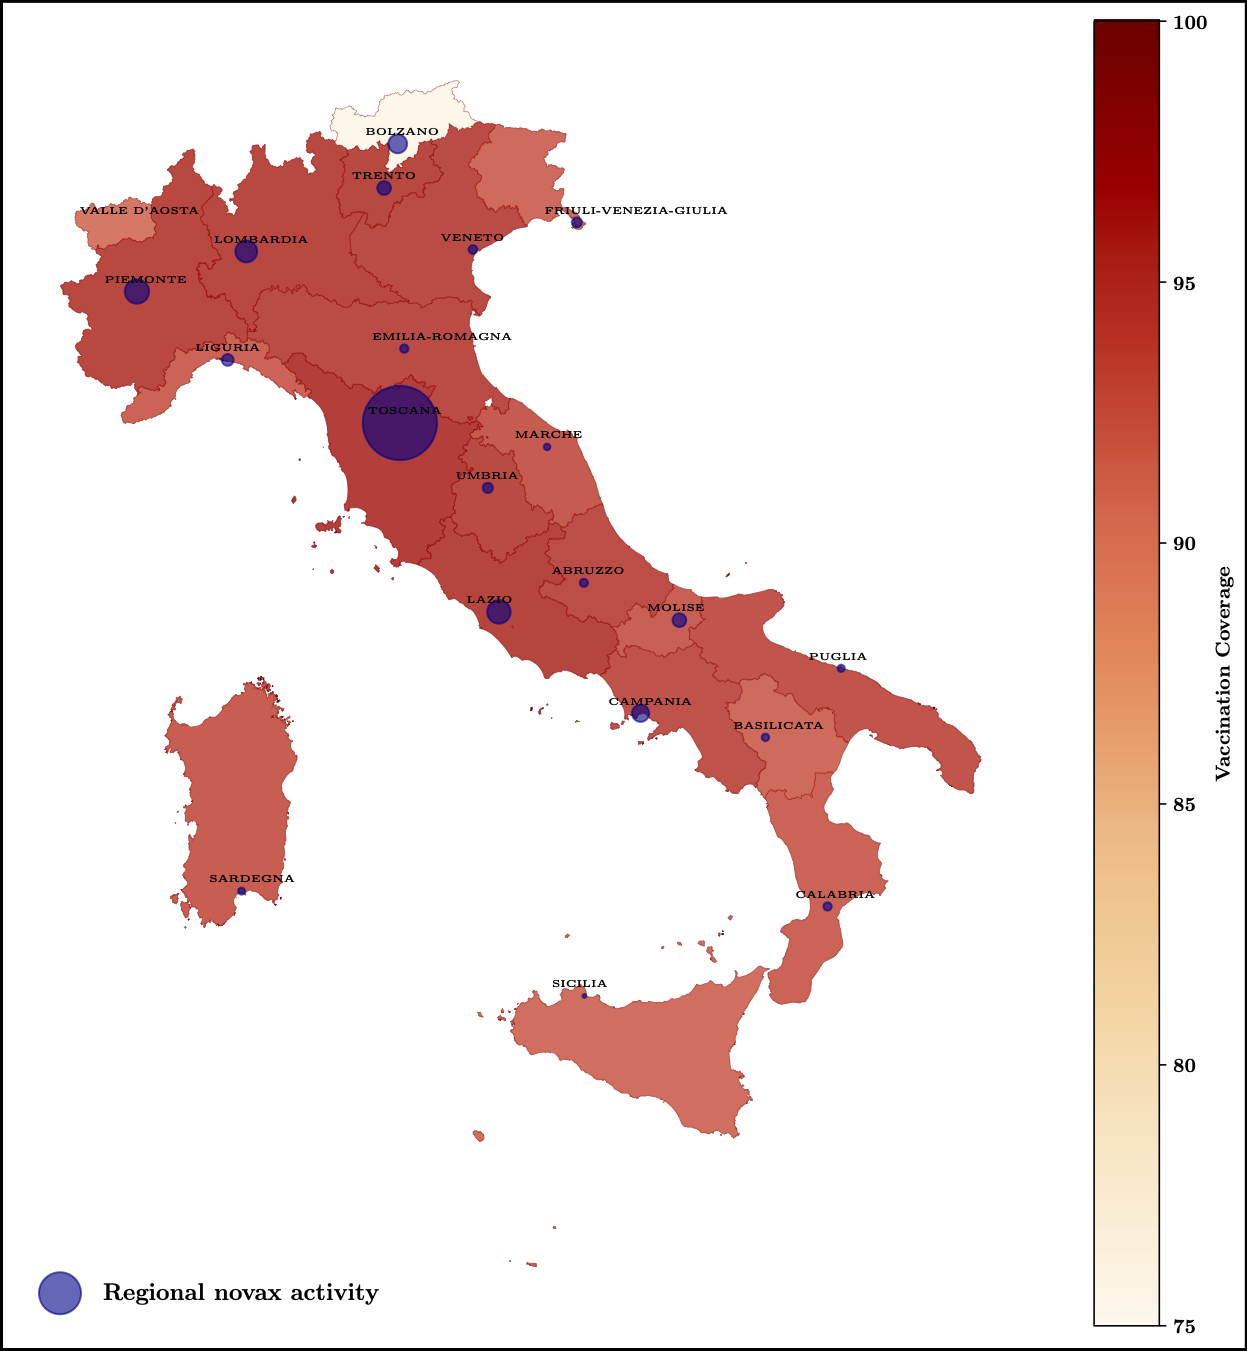
\includegraphics[width=0.8\textwidth]{Paper_template/image/map/map_2020.pdf} \label{fig:map_result_d} }
	\end{minipage}
	\caption{\label{fig:map_result} Superposition maps of measles vaccination coverage (shades of red) and novax activity on Twitter (blue points with radius proportional to its weight). The years under analysis are 2017-2020. Vaccination coverage for 2020 is not available, so, in 2020 map, 2019 vaccination coverage is used.}
	\end{figure*}
    
In Tab. \ref{tab:vaxcoverage} the data regarding measles vaccination coverage of the years 2017-2019 \cite{ministerosalute} are reported. The national average has increased over these three years, certainly thanks to the 2017 vaccination plan presented in the Lorenzin Decree (Sec. \ref{sec:introduction}). Sicilia and Friuli Venezia Giulia grew by up to 6-7 percentage points, but have not  reached the minimum threshold recommended by the World Health Organization yet. This threshold is set at 95$\%$ \cite{ministerosalute} and half of the Italian regions have overcame it. On the contrary, the autonomous province of Bolzano, stands out being the only area 20 points below with respect to the national average.


In Fig. \ref{fig:map_result} is reported a superposition of vaccination coverage and novax opinions measure results. Through these maps, one can note that there is no evident correspondence between a low vaccination coverage and a high novax twitter activity. For example the autonomous province of Bolzano has by far the lowest vaccination coverage, but there is no greater amount of novax ideas on Twitter than in the rest of Italy. This result could certainly resemble the real situation, but, to confirm it, an analysis carried out with an higher number of data, by order of magnitudes, would be required. Indeed, we are far from capture the whole novax activity on twitter and these maps show only the relative distribution with respect to our data. However, a clearly visible hub is present in Toscana almost every year and in general the most of the measured activity concentrate in the northern regions, especially in Toscana, Emilia Romagna and Veneto. Especially, in Toscana and Veneto this could be due to the two local novax associations “@clivatoscana” and “@corvelva” which are very active on Twitter, as observed in the semantic analysis. Finally, we can say that the effects of a legislative measure such as the Lorenzin decree seems independent of the novax activity in a specific region. Also Covid-19 effects are not so evident in the 2020 map. However, to confirm this hypothesis with a meaningful confidence level, higher number of data by order of magnitudes would have been required.




\section{Conclusions}
\label{sec:conclusions}

In this work, we analyze the distribution of novax opinions in Italy in the time interval 2017-2020 by means of tweets with clearly anti-vaccine content. From a semantic analysis, it emerges that there are some super spreaders who frequently create original tweets, that are retweeted by the majority. However, in 2020 there is an higher number of unique users which are also different with respect to the others years. This could be a consequence of Covid-19 pandemic: people feel vaccination as a closer topic and many more users express their doubts and oppositions. 
Moreover, from the provenience of the collected tweets, we make a geographical map of novax opinions in Italy by assigning a weight to each region. 
%We assign a weight to each user depending of the number of its tweet, the like and the retweets he receives; summing all the users weights from a region we obtain a region weight of anti-vaccine opinions. 
It results that especially Toscana, Emilia Romagna and Veneto have novax high concentrations, mostly due to local super spreaders. 
The distribution of novax opinions on the Italian territory does not seem to have changed relevantly over the years and looks unaffected by Lorenzin Decree on vaccination and by Covid-19. Finally, we do not find a correspondence between low coverage and novax hubs.
%: the Autonomous province of Bolzano has by far the lowest vaccination coverage, but there is no greater amount of novax ideas on Twitter than in the rest of Italy.
However, to confirm all these hypothesis with a meaningful confidence level, many more data would have been required.

To conclude, as a future analysis, it would be interesting and useful to make a coarse graining by province of origin, but, for this purpose, even more data are needed. 
A such big data collection is indeed worthy. Mining and localizing opinions from social networks has a great relevance: this type of analysis can be useful in identifying hubs of anti-vaccination ideas and consequently in choosing where to invest resources for public opinion awareness campaigns on vaccination.



% To add bibliography (file references.bib)
\bibliographystyle{unsrt}
\bibliography{references}{}
%\printbibliography

\end{document}
